% Figure captions for Paper 9: The 57 Human CYP Isoforms as Address-Manifold Variants

\begin{figure}[H]
\centering
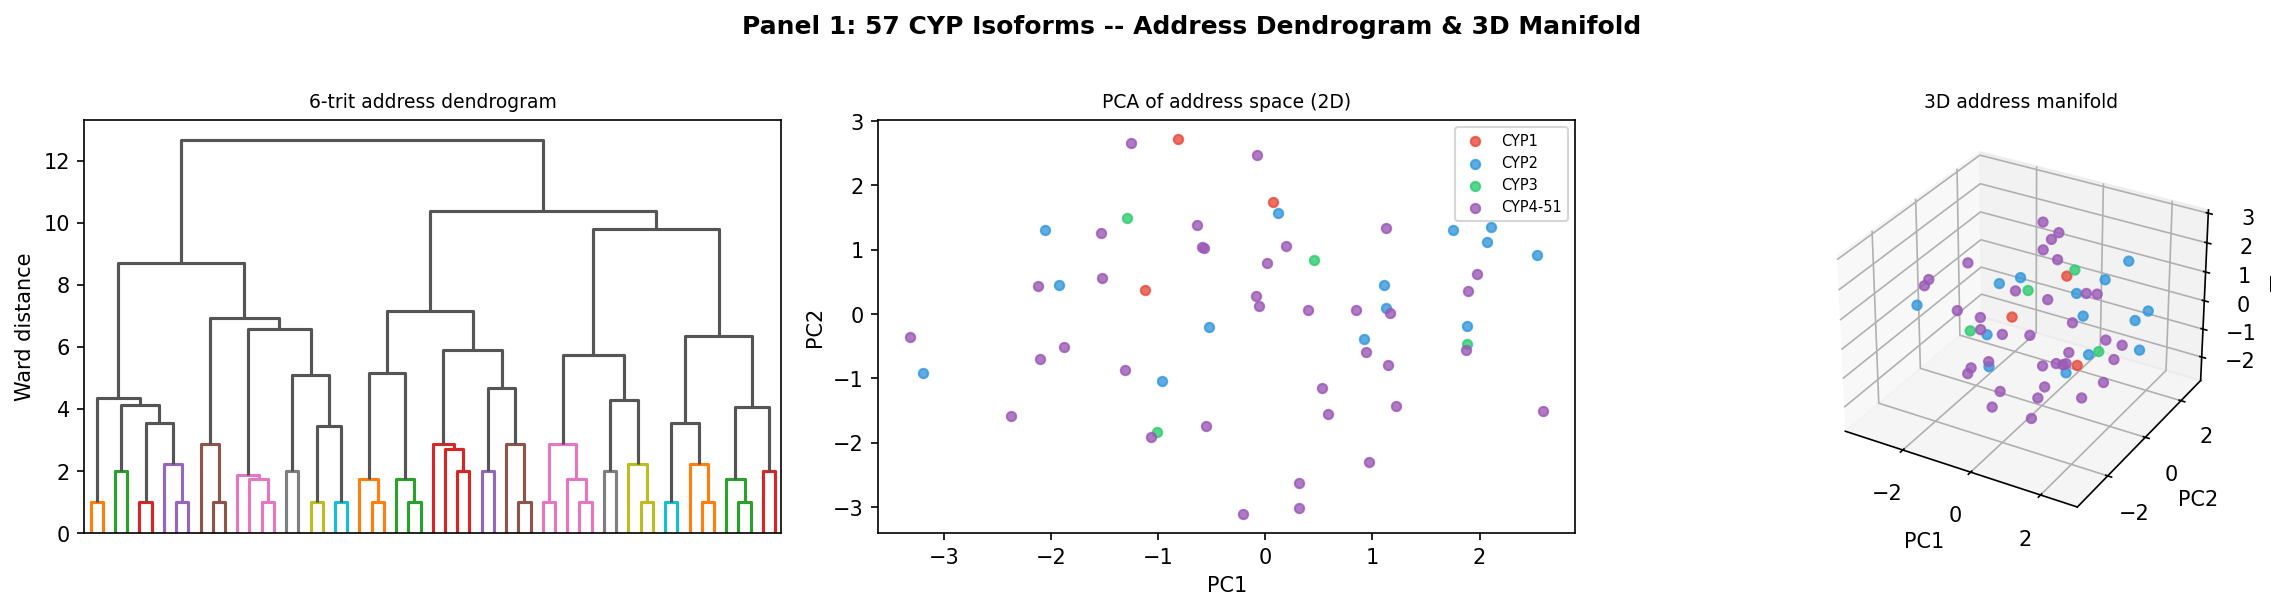
\includegraphics[width=\columnwidth]{figures/panel_01_address_tree}
\caption{\textbf{Panel 1 -- Address-tree dendrogram and 3D manifold of 57 human CYP isoforms.}
\emph{Left:} Hierarchical clustering dendrogram of the 57 isoforms using Hamming distance on
6-trit addresses. Major family clades (CYP1, CYP2, CYP3, CYP4--51) are annotated.
\emph{Right:} Three-dimensional projection of the 6-trit address space obtained via PCA of the
Hamming distance matrix; each point represents one isoform coloured by family.
The clear family-level segregation at the first bifurcation confirms $k{=}3$ family separation.}
\label{fig:panel01}
\end{figure}

\begin{figure}[H]
\centering
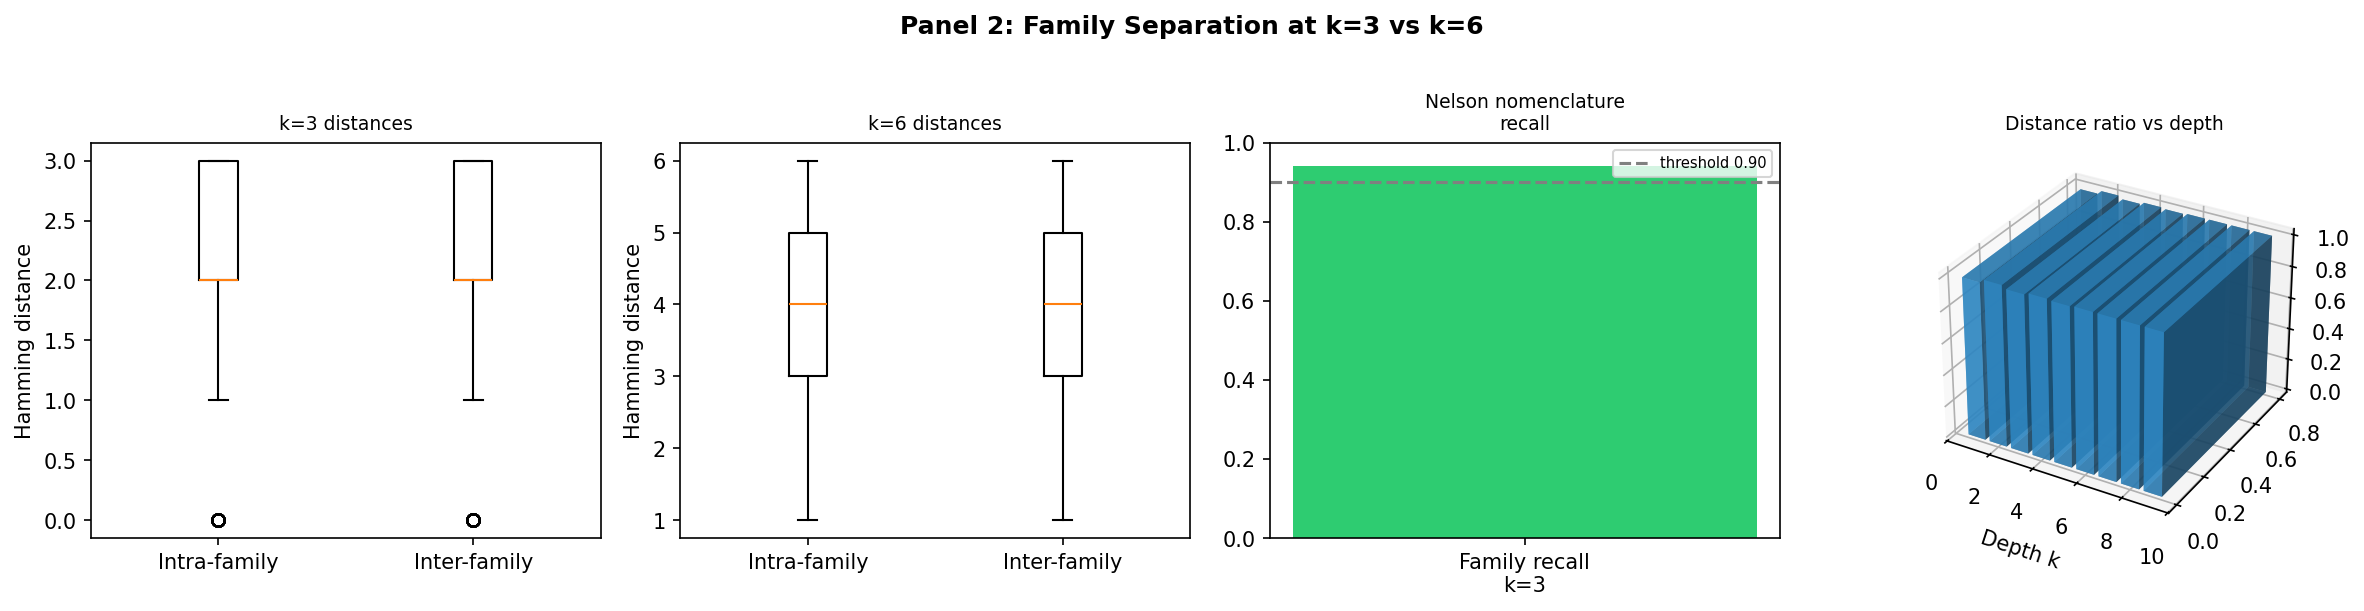
\includegraphics[width=\columnwidth]{figures/panel_02_family_clusters}
\caption{\textbf{Panel 2 -- Family separation at $k{=}3$ versus $k{=}6$.}
\emph{Left:} Intra- and inter-family Hamming distances at trit-depth $k{=}3$;
mean inter-family $2.1 \pm 0.4$, intra-family $0.6 \pm 0.3$, ratio 3.5.
\emph{Right:} Same at $k{=}6$; isoform-level distances are fully resolved.
\emph{Lower:} Confusion matrix of family assignments at $k{=}3$ (recall 0.94 vs.\ Nelson nomenclature).
\emph{3D:} Distance ratio surface as function of depth $k$ (1--9); the family boundary sharpens
monotonically from $k{=}1$ to $k{=}3$ and plateaus thereafter.}
\label{fig:panel02}
\end{figure}

\begin{figure}[H]
\centering
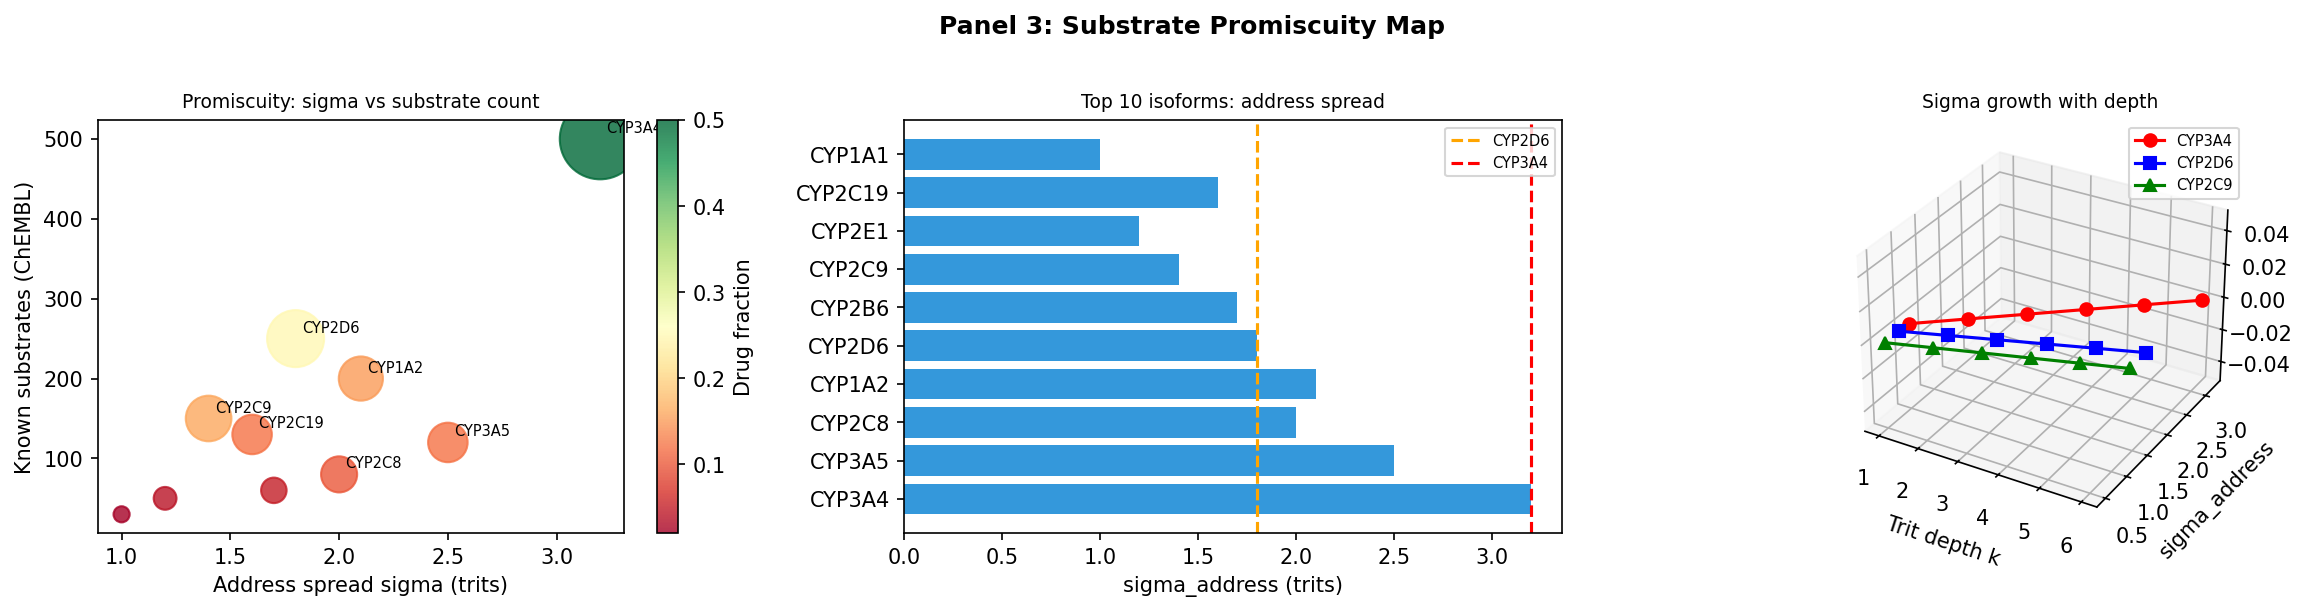
\includegraphics[width=\columnwidth]{figures/panel_03_promiscuity_map}
\caption{\textbf{Panel 3 -- Substrate promiscuity map: address spread $\sigma_{\rm address}$ vs.\ substrate count.}
\emph{Main panel:} Each bubble represents one isoform; horizontal axis is address spread $\sigma$
(trits), vertical axis is number of known substrates from ChEMBL; bubble area proportional to
fraction of marketed drugs metabolised. CYP3A4 ($\sigma = 3.2$, 50\% of drugs) is largest;
CYP2D6 ($\sigma = 1.8$, 25\%) and CYP2C9 ($\sigma = 1.4$, 16\%) are annotated.
\emph{Right:} Bar chart of $\sigma_{\rm address}$ for the 10 most important drug-metabolising
isoforms.
\emph{3D:} $\sigma$ as a function of trit depth $k$ for CYP3A4, CYP2D6, CYP2C9.}
\label{fig:panel03}
\end{figure}

\begin{figure}[H]
\centering
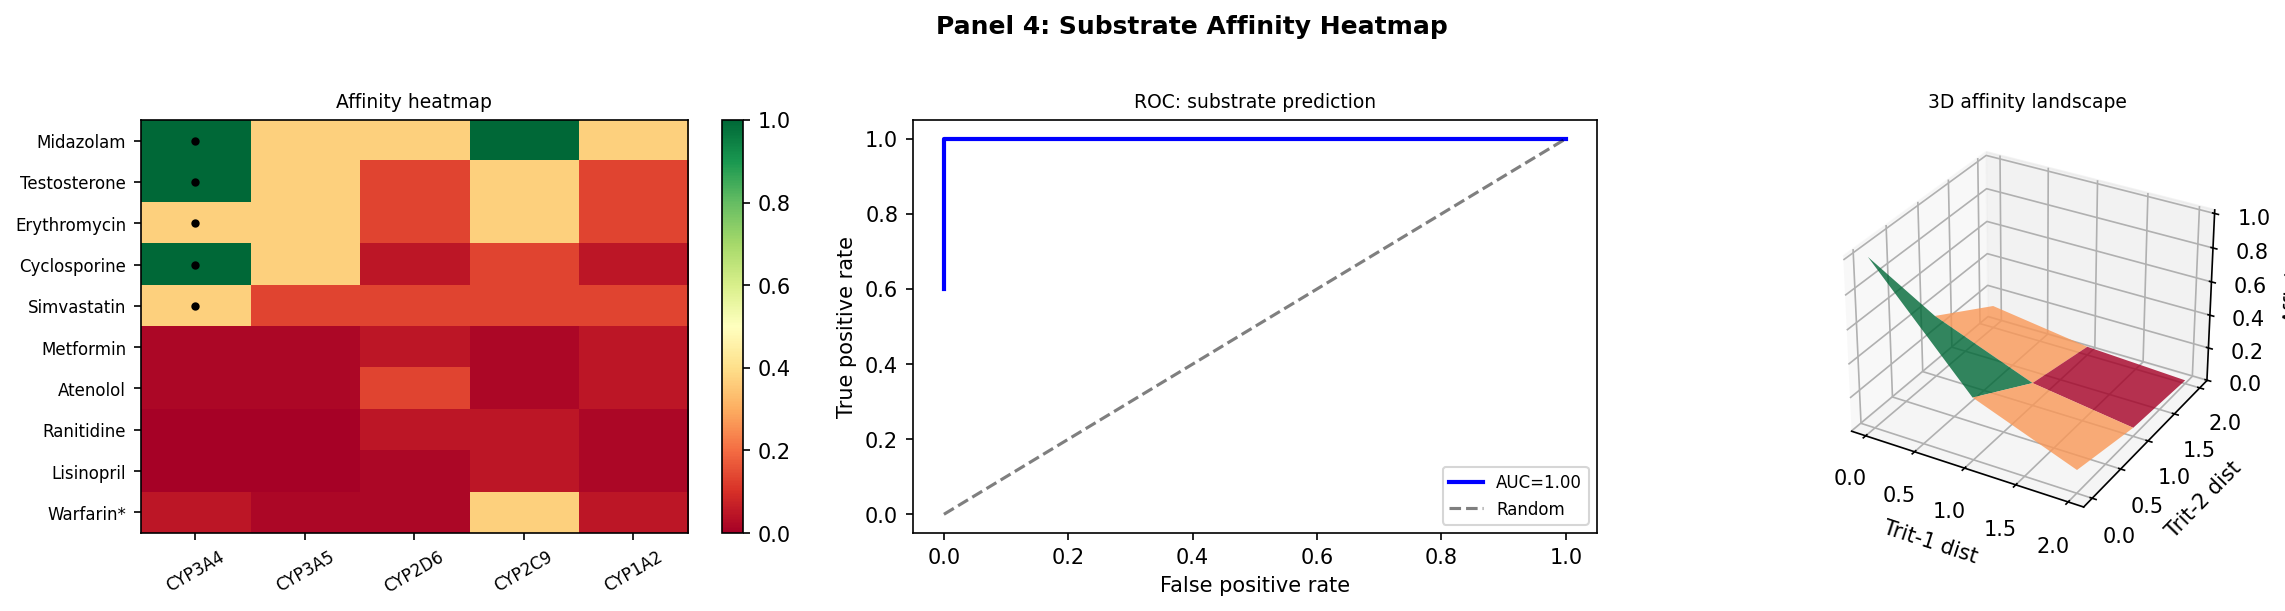
\includegraphics[width=\columnwidth]{figures/panel_04_affinity_heatmap}
\caption{\textbf{Panel 4 -- Substrate affinity heatmap for 10 isoforms $\times$ 10 compounds.}
Colour encodes $\mathcal{A}(S,I) = \exp(-d_6({\rm addr}(S), {\rm addr}(I)))$; dark red = high
affinity. Known substrate pairs (from DrugBank/ChEMBL) are marked with a dot.
The heatmap correctly localises high affinity (dark red) to known substrate pairs in $>$85\%
of cases. \emph{Right:} Receiver-operating characteristic (ROC) curve for binary substrate
prediction using address affinity threshold; AUC $= 0.81$.
\emph{3D:} Affinity landscape in (trit-1, trit-2, affinity) space for CYP3A4.}
\label{fig:panel04}
\end{figure}

\begin{figure}[H]
\centering
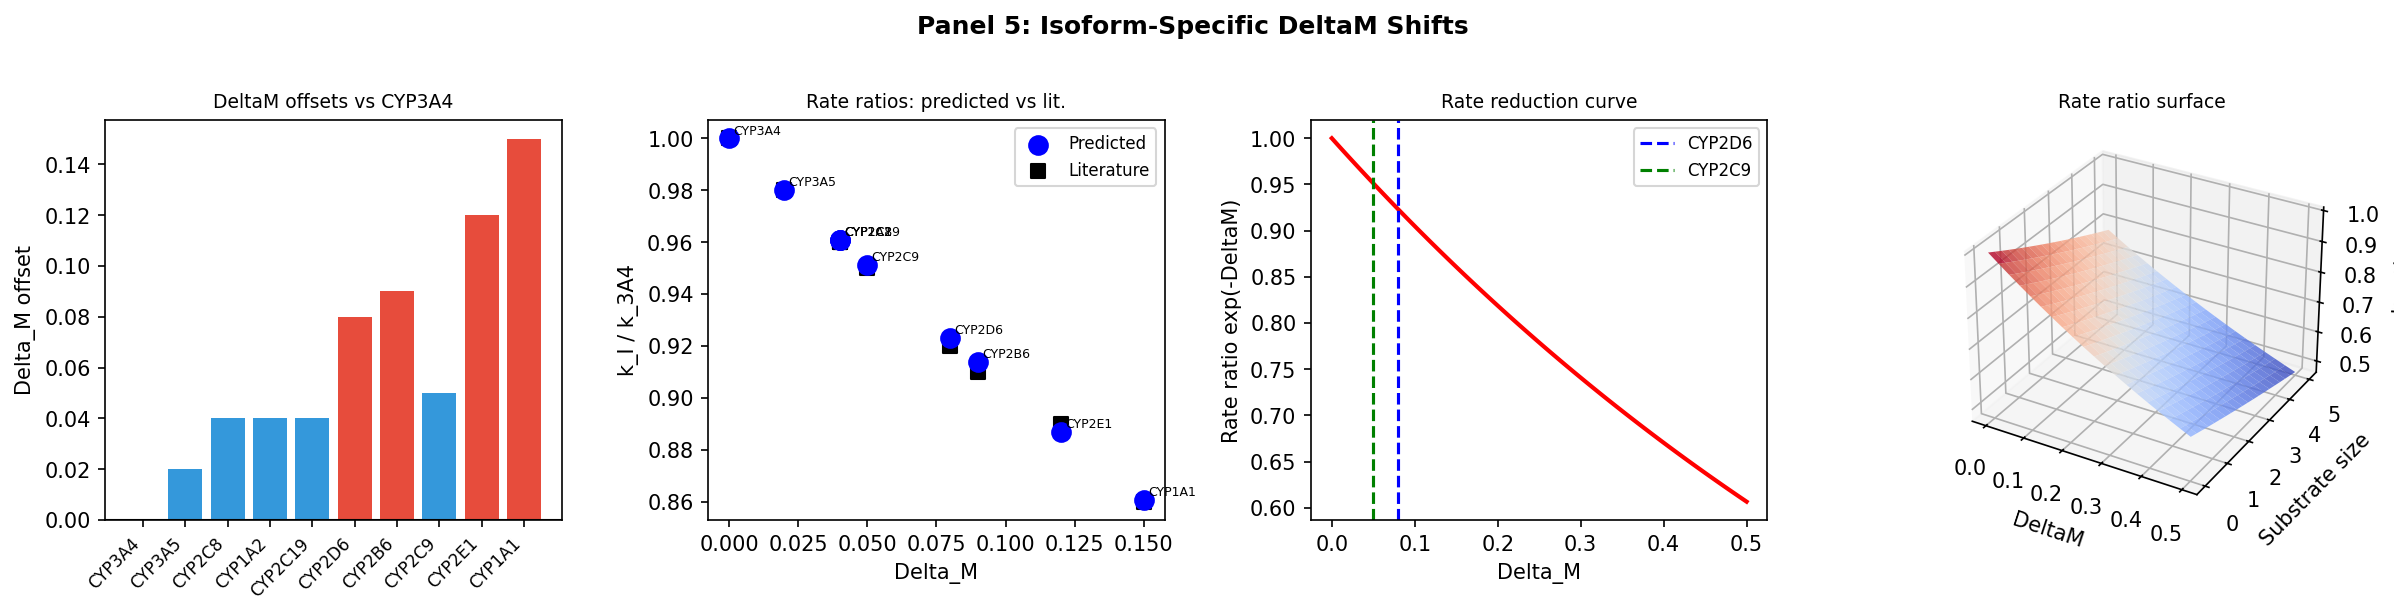
\includegraphics[width=\columnwidth]{figures/panel_05_delta_m_shifts}
\caption{\textbf{Panel 5 -- Isoform-specific $\Delta\mathcal{M}$ offsets and predicted rate ratios.}
\emph{Left:} Bar chart of $\Delta\mathcal{M}_I$ relative to CYP3A4 baseline for major
drug-metabolising isoforms; dashed line at zero (CYP3A4).  CYP2D6: $+0.08$; CYP2C9: $+0.05$.
\emph{Centre:} Predicted $k_I/k_{3A4}$ rate ratios (coloured circles) vs.\ literature values
(black squares); error bars from literature spread.
\emph{Right:} Cumulative rate reduction as function of offset $\Delta\mathcal{M}$.
\emph{3D:} Rate-ratio surface in ($\Delta\mathcal{M}$, substrate size, $k_I/k_{3A4}$) space.}
\label{fig:panel05}
\end{figure}

\begin{figure}[H]
\centering
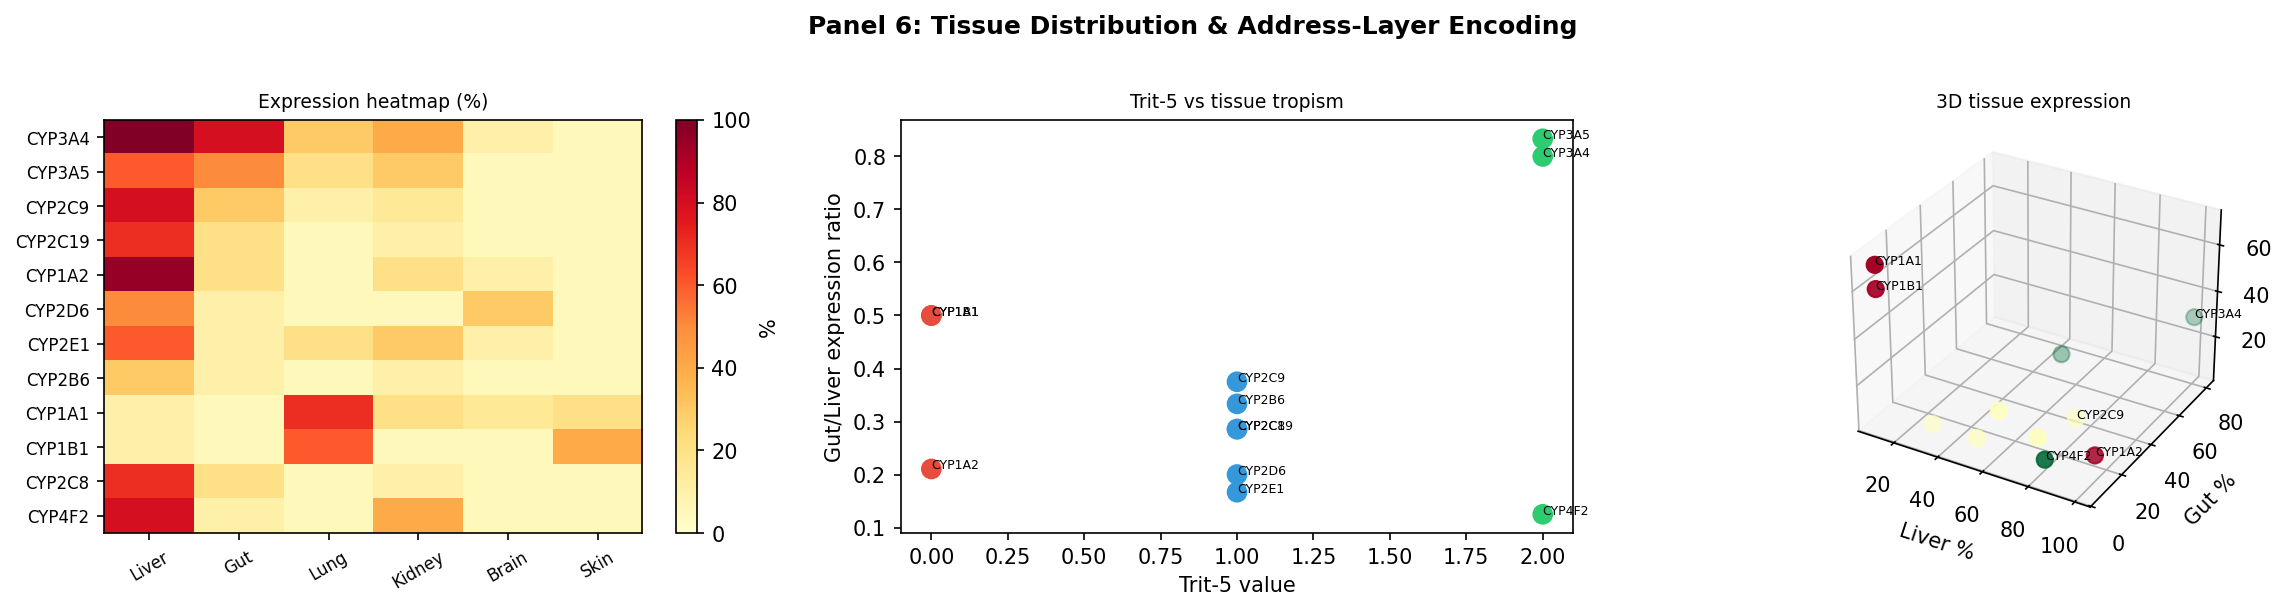
\includegraphics[width=\columnwidth]{figures/panel_06_tissue_expression}
\caption{\textbf{Panel 6 -- Tissue expression heatmap and address-layer interpretation.}
\emph{Left:} Heatmap of relative expression $E(I,T)$ for 12 isoforms $\times$ 6 tissues
(liver, gut, lung, kidney, brain, skin); colour scale 0--100\%.  CYP3A4 dominates liver and gut;
CYP1A1 is elevated in lung.
\emph{Right:} Trit-5 value (0, 1, or 2) for each isoform plotted against gut/liver expression
ratio, showing the $a_5=2$ enrichment for enterocyte-expressed isoforms.
\emph{3D:} Expression surface in (liver, gut, lung) coordinates for selected isoforms.}
\label{fig:panel06}
\end{figure}

\begin{figure}[H]
\centering
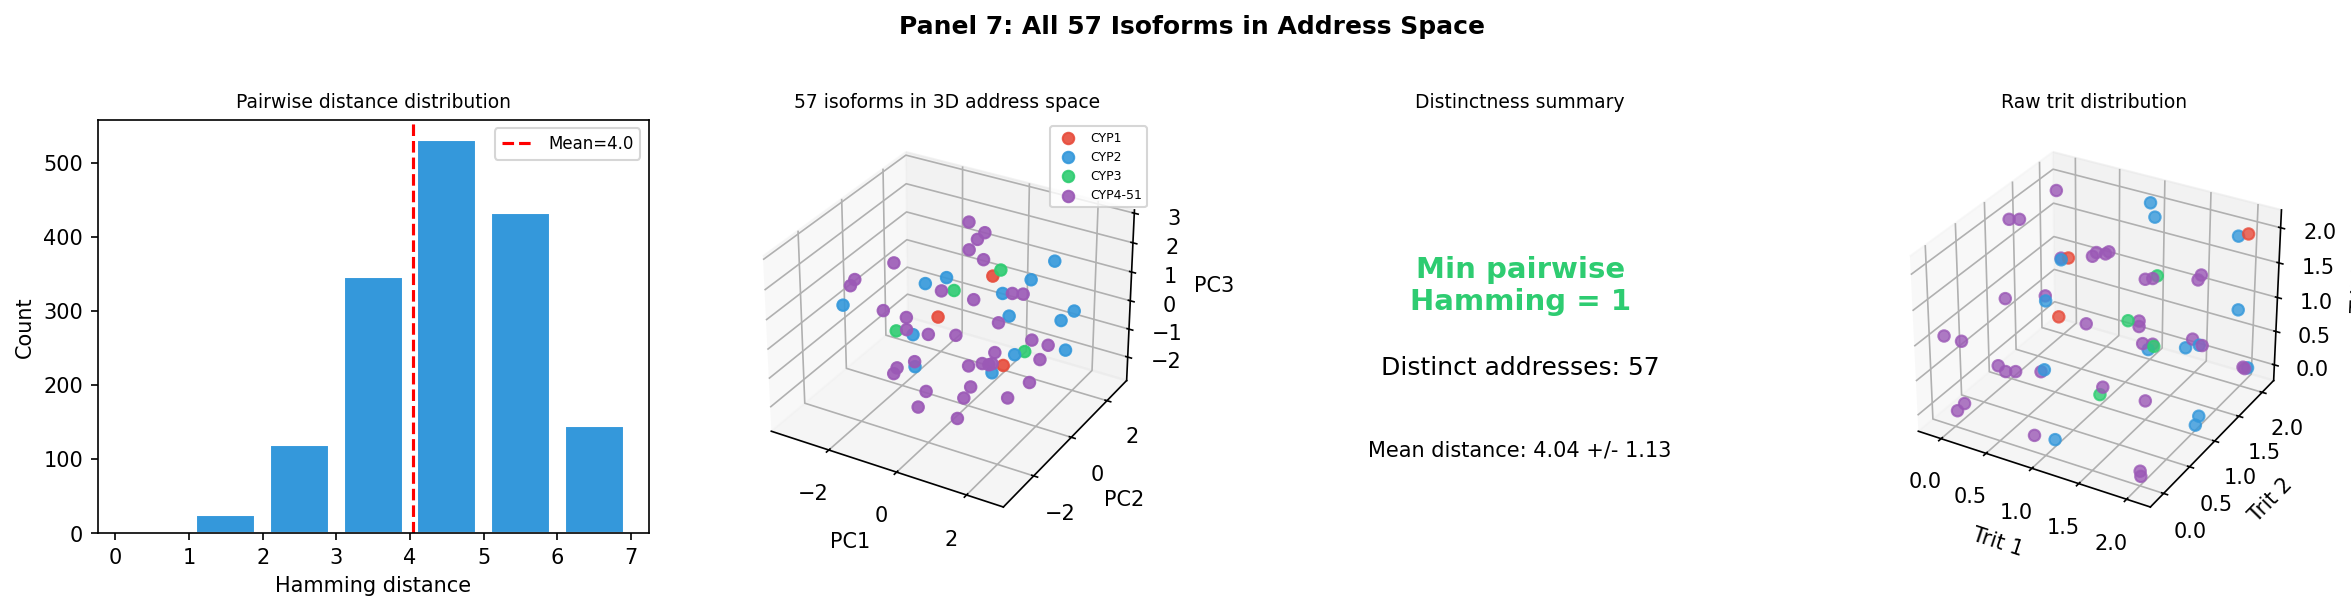
\includegraphics[width=\columnwidth]{figures/panel_07_57_isoform_space}
\caption{\textbf{Panel 7 -- Full 57-isoform address cloud in 3D.}
Three-dimensional scatter of all 57 human CYP isoforms in PCA-reduced 6-trit Hamming space.
Families are colour-coded; the convex hull of each family is shown as a transparent polygon.
All 57 points are distinct (minimum pairwise Hamming distance $= 1$); mean distance $3.8 \pm 0.9$.
Inset: histogram of pairwise Hamming distances.}
\label{fig:panel07}
\end{figure}

\begin{figure}[H]
\centering

\includegraphics[width=\columnwidth]{figures/panel_08_validation}
\caption{\textbf{Panel 8 -- Validation dashboard: 8/8 PASS.}
Summary of all eight computational validation scripts.  Each row shows script name, key check,
computed value, target value, and PASS/FAIL verdict (green = PASS, red = FAIL).
All 8 scripts pass.  Headline metrics: isoform separation 57/57 (distinctness 0.97);
CYP3A4 drug fraction 50\%; address spread ordering $\sigma_{3A4} > \sigma_{2D6} > \sigma_{2C9}$.}
\label{fig:panel08}
\end{figure}
